\chapter{Sistemas lineales de ecuaciones diferenciales}\label{sistemasedos}

\section{Sistemas de primer orden y notación matricial}

\subsection{Forma general y notación vectorial}

Un \emph{sistema lineal de primer orden} de $n$ ecuaciones diferenciales para las funciones incógnita $x_1(t),\dots,x_n(t)$ tiene la forma
\begin{equation}
\begin{aligned}
x_1' &= a_{11}(t)x_1 + a_{12}(t)x_2 + \cdots + a_{1n}(t)x_n + f_1(t),\\
x_2' &= a_{21}(t)x_1 + a_{22}(t)x_2 + \cdots + a_{2n}(t)x_n + f_2(t),\\
&\vdots\\
x_n' &= a_{n1}(t)x_1 + a_{n2}(t)x_2 + \cdots + a_{nn}(t)x_n + f_n(t),
\end{aligned}
\end{equation}
donde $a_{ij}(t)$ y $f_i(t)$ son funciones continuas en un intervalo $I$.

Si definimos el vector columna
\[
\mathbf{X}(t)=
\begin{pmatrix}
x_1(t)\\x_2(t)\\\vdots\\x_n(t)
\end{pmatrix},\qquad
\mathbf{F}(t)=
\begin{pmatrix}
f_1(t)\\f_2(t)\\\vdots\\f_n(t)
\end{pmatrix},
\]
y la matriz de coeficientes
\[
A(t)=
\begin{pmatrix}
a_{11}(t)&a_{12}(t)&\cdots&a_{1n}(t)\\
a_{21}(t)&a_{22}(t)&\cdots&a_{2n}(t)\\
\vdots&\vdots&\ddots&\vdots\\
a_{n1}(t)&a_{n2}(t)&\cdots&a_{nn}(t)
\end{pmatrix},
\]
el sistema se escribe de manera compacta como
\begin{equation}
\mathbf{X}'(t)=A(t)\mathbf{X}(t)+\mathbf{F}(t).
\end{equation}

Cuando $\mathbf{F}(t)\equiv \mathbf{0}$, el sistema se llama \emph{homogéneo}; en caso contrario, \emph{no homogéneo}. Si la matriz $A$ es constante, el sistema es de \emph{coeficientes constantes}.

\begin{definition}
Una \emph{solución} del sistema en un intervalo $I$ es un vector de funciones $\mathbf{X}(t)$ diferenciable en $I$ que satisface la ecuación para todo $t\in I$. Dado un punto inicial $t_0\in I$ y un vector $\mathbf{X}_0\in\mathbb{R}^n$, el \emph{problema de valor inicial (PVI)} consiste en encontrar una solución que cumpla $\mathbf{X}(t_0)=\mathbf{X}_0$.
\end{definition}

\subsection{Reescritura de una EDO de orden $n$ como sistema}

Cualquier ecuación diferencial ordinaria lineal de orden $n$,
\[
y^{(n)}+p_{n-1}(t)y^{(n-1)}+\cdots+p_1(t)y'+p_0(t)y=g(t),
\]
puede transformarse en un sistema de $n$ ecuaciones de primer orden mediante el cambio de variables
\[
x_1=y,\quad x_2=y',\quad x_3=y'',\quad \dots,\quad x_n=y^{(n-1)}.
\]
Entonces $x_1'=x_2,\; x_2'=x_3,\;\dots,\; x_{n-1}'=x_n$, y la última ecuación se obtiene despejando $y^{(n)}$:
\[
x_n'=y^{(n)}=-p_0(t)x_1-p_1(t)x_2-\cdots-p_{n-1}(t)x_n+g(t).
\]

\begin{example}[Conversión de una EDO de segundo orden a sistema]
Convertir la ecuación $y''-3y'+2y=0$ en un sistema de primer orden.
\begin{myproof}
\textbf{Paso 1.} Definir las nuevas variables:
\[
x_1=y,\qquad x_2=y'.
\]

\textbf{Paso 2.} Escribir las derivadas:
\[
x_1'=x_2,\qquad x_2'=y''=3y'-2y=3x_2-2x_1.
\]

\textbf{Paso 3.} Expresar en forma matricial:
\[
\begin{pmatrix}
x_1'\\x_2'
\end{pmatrix}
=
\begin{pmatrix}
0&1\\
-2&3
\end{pmatrix}
\begin{pmatrix}
x_1\\x_2
\end{pmatrix}.
\]

\textbf{Respuesta final:} El sistema equivalente es
\[
\boxed{
\mathbf{X}'=
\begin{pmatrix}
0&1\\
-2&3
\end{pmatrix}
\mathbf{X},\quad
\mathbf{X}=
\begin{pmatrix}
x_1\\x_2
\end{pmatrix}
}
\]
\end{myproof}
\end{example}

\begin{example}[Conversión de una EDO no homogénea de tercer orden]
Escribir el sistema asociado a $y'''-2y''+y'-4y=t e^t$.
\begin{myproof}
\textbf{Paso 1.} Definir $x_1=y,\; x_2=y',\; x_3=y''$.

\textbf{Paso 2.} Las derivadas son:
\[
x_1'=x_2,\quad x_2'=x_3,\quad x_3'=y'''=2y''-y'+4y+t e^t=2x_3-x_2+4x_1+t e^t.
\]

\textbf{Paso 3.} Escribir el sistema:
\[
\begin{cases}
x_1'=x_2,\\
x_2'=x_3,\\
x_3'=4x_1-x_2+2x_3+t e^t.
\end{cases}
\]

\textbf{Paso 4.} Forma matricial:
\[
\mathbf{X}'=
\begin{pmatrix}
0&1&0\\
0&0&1\\
4&-1&2
\end{pmatrix}
\mathbf{X}
+
\begin{pmatrix}
0\\0\\t e^t
\end{pmatrix}.
\]

\textbf{Respuesta final:}
\[
\boxed{
\mathbf{X}'=
\begin{pmatrix}
0&1&0\\
0&0&1\\
4&-1&2
\end{pmatrix}
\mathbf{X}
+
\begin{pmatrix}
0\\0\\t e^t
\end{pmatrix},\quad
\mathbf{X}=
\begin{pmatrix}
x_1\\x_2\\x_3
\end{pmatrix}
}
\]
\end{myproof}
\end{example}

\section{Método de eliminación (reducción a una EDO de orden superior)}

Para sistemas $2\times2$ de la forma
\[
\begin{cases}
x' = a_{11}x + a_{12}y + f_1(t),\\
y' = a_{21}x + a_{22}y + f_2(t),
\end{cases}
\]
podemos eliminar una de las variables derivando una ecuación y sustituyendo en la otra, obteniendo una EDO lineal de segundo orden para la variable restante.

\begin{example}[Método de eliminación, sistema homogéneo]
Resolver el sistema
\[
\begin{cases}
x' = x + 2y,\\
y' = 3x + 2y.
\end{cases}
\]
\begin{myproof}
\textbf{Paso 1.} Despejar $y$ de la primera ecuación:
\[
y=\frac{x'-x}{2}.
\]

\textbf{Paso 2.} Derivar esta expresión:
\[
y'=\frac{x''-x'}{2}.
\]

\textbf{Paso 3.} Sustituir en la segunda ecuación:
\[
\frac{x''-x'}{2}=3x+2\left(\frac{x'-x}{2}\right)=3x+x'-x=2x+x'.
\]
Multiplicando por 2:
\[
x''-x'=4x+2x' \implies x''-3x'-4x=0.
\]

\textbf{Paso 4.} Resolver la EDO de segundo orden. La ecuación característica es $r^2-3r-4=0$ con raíces $r=4$ y $r=-1$. Luego
\[
x(t)=c_1 e^{4t}+c_2 e^{-t}.
\]

\textbf{Paso 5.} Despejar $y$:
\[
y=\frac{x'-x}{2}
=\frac{4c_1 e^{4t}-c_2 e^{-t} - (c_1 e^{4t}+c_2 e^{-t})}{2}
=\frac{3c_1 e^{4t}-2c_2 e^{-t}}{2}.
\]

\textbf{Respuesta final:}
\[
\boxed{
x(t)=c_1 e^{4t}+c_2 e^{-t},\qquad
y(t)=\frac{3}{2}c_1 e^{4t}-c_2 e^{-t}
}
\]
\end{myproof}
\end{example}

\begin{example}[Método de eliminación, sistema no homogéneo]
Resolver
\[
\begin{cases}
x' = -x + y + 1,\\
y' = -x - y + 2t.
\end{cases}
\]
\begin{myproof}
\textbf{Paso 1.} Despejar $y$ de la primera: $y=x'+x-1$.

\textbf{Paso 2.} Derivar: $y'=x''+x'$.

\textbf{Paso 3.} Sustituir en la segunda:
\[
x''+x'=-x-(x'+x-1)+2t=-2x-x'+1+2t.
\]
Entonces $x''+2x'+2x=1+2t$.

\textbf{Paso 4.} Resolver la EDO lineal no homogénea. La solución homogénea: $x_h=e^{-t}(c_1\cos t+c_2\sen t)$. Buscamos una particular de la forma $x_p=At+B$. Sustituyendo:
\[
0+2A+2(At+B)=1+2t \implies 2At+(2A+2B)=1+2t.
\]
Comparando: $2A=2\Rightarrow A=1$; $2+2B=1\Rightarrow B=-\frac12$. Luego $x_p=t-\frac12$.
Por tanto,
\[
x(t)=e^{-t}(c_1\cos t+c_2\sen t)+t-\frac12.
\]

\textbf{Paso 5.} Calcular $y=x'+x-1$:
\[
x'=e^{-t}[(c_2-c_1)\cos t-(c_1+c_2)\sen t]+1,
\]
luego
\[
y= e^{-t}[(c_2-c_1)\cos t-(c_1+c_2)\sen t]+1 + e^{-t}(c_1\cos t+c_2\sen t)+t-\frac12 -1
\]
simplificando:
\[
y=e^{-t}[c_2\cos t-c_1\sen t]+t-\frac12.
\]

\textbf{Respuesta final:}
\[
\boxed{
x(t)=e^{-t}(c_1\cos t+c_2\sen t)+t-\frac12,\qquad
y(t)=e^{-t}(c_2\cos t-c_1\sen t)+t-\frac12
}
\]
\end{myproof}
\end{example}

\section{Sistemas homogéneos con coeficientes constantes: $\mathbf{X}'=A\mathbf{X}$}

Consideremos el sistema homogéneo con $A\in\mathbb{R}^{n\times n}$ constante:
\[
\mathbf{X}'=A\mathbf{X}.
\]
Buscamos soluciones de la forma $\mathbf{X}=e^{\lambda t}\mathbf{v}$, con $\mathbf{v}\neq 0$. Sustituyendo:
\[
\lambda e^{\lambda t}\mathbf{v}=A e^{\lambda t}\mathbf{v} \implies (A-\lambda I)\mathbf{v}=0.
\]
Por tanto, $\lambda$ debe ser un valor propio de $A$ y $\mathbf{v}$ un vector propio asociado.

\begin{theorem}
Si $A$ tiene $n$ vectores propios linealmente independientes $\mathbf{v}_1,\dots,\mathbf{v}_n$ correspondientes a los valores propios $\lambda_1,\dots,\lambda_n$ (no necesariamente distintos), entonces la solución general del sistema homogéneo es
\[
\mathbf{X}(t)=c_1 e^{\lambda_1 t}\mathbf{v}_1+c_2 e^{\lambda_2 t}\mathbf{v}_2+\cdots+c_n e^{\lambda_n t}\mathbf{v}_n.
\]
\end{theorem}

\subsection{Caso 1: Valores propios reales distintos}

Cuando los valores propios son reales y todos diferentes, la matriz $A$ es diagonalizable y la fórmula anterior proporciona la solución general.

\begin{example}[Valores propios reales distintos, sistema 2x2]
Resolver $\mathbf{X}'=
\begin{pmatrix}
1&2\\
3&2
\end{pmatrix}\mathbf{X}$.
\begin{myproof}
\textbf{Paso 1.} Calcular valores propios:
\[
\det(A-\lambda I)=
\begin{vmatrix}
1-\lambda&2\\
3&2-\lambda
\end{vmatrix}
=(1-\lambda)(2-\lambda)-6=\lambda^2-3\lambda-4=(\lambda-4)(\lambda+1).
\]
Raíces: $\lambda_1=4,\; \lambda_2=-1$.

\textbf{Paso 2.} Vectores propios.
Para $\lambda_1=4$: $(A-4I)\mathbf{v}=0$:
\[
\begin{pmatrix}
-3&2\\
3&-2
\end{pmatrix}
\begin{pmatrix}
v_1\\v_2
\end{pmatrix}=0
\Rightarrow -3v_1+2v_2=0\Rightarrow v_2=\frac32 v_1.
\]
Tomamos $\mathbf{v}_1=(2,3)^T$.

Para $\lambda_2=-1$: $(A+I)\mathbf{v}=0$:
\[
\begin{pmatrix}
2&2\\
3&3
\end{pmatrix}
\begin{pmatrix}
v_1\\v_2
\end{pmatrix}=0
\Rightarrow v_1+v_2=0\Rightarrow v_2=-v_1.
\]
Tomamos $\mathbf{v}_2=(1,-1)^T$.

\textbf{Paso 3.} Escribir la solución general:
\[
\mathbf{X}=c_1 e^{4t}\begin{pmatrix}2\\3\end{pmatrix}+c_2 e^{-t}\begin{pmatrix}1\\-1\end{pmatrix}.
\]

\textbf{Respuesta final:}
\[
\boxed{
\mathbf{X}(t)=c_1 e^{4t}
\begin{pmatrix}
2\\3
\end{pmatrix}
+c_2 e^{-t}
\begin{pmatrix}
1\\-1
\end{pmatrix}
}
\]
\end{myproof}
\end{example}

\begin{example}[Valores propios reales distintos, sistema 3x3]
Resolver $\mathbf{X}'=
\begin{pmatrix}
1&0&0\\
2&2&0\\
3&4&3
\end{pmatrix}\mathbf{X}$.
\begin{myproof}
\textbf{Paso 1.} La matriz es triangular superior, así que los valores propios son los elementos de la diagonal: $\lambda_1=1,\lambda_2=2,\lambda_3=3$.

\textbf{Paso 2.} Vectores propios.
Para $\lambda_1=1$: $(A-I)\mathbf{v}=0$:
\[
\begin{pmatrix}
0&0&0\\
2&1&0\\
3&4&2
\end{pmatrix}
\begin{pmatrix}
v_1\\v_2\\v_3
\end{pmatrix}=0
\Rightarrow
\begin{cases}
2v_1+v_2=0\\
3v_1+4v_2+2v_3=0
\end{cases}
\Rightarrow v_2=-2v_1,\; v_3=\frac{5}{2}v_1.
\]
Tomamos $\mathbf{v}_1=(2,-4,5)^T$.

Para $\lambda_2=2$: $(A-2I)\mathbf{v}=0$:
\[
\begin{pmatrix}
-1&0&0\\
2&0&0\\
3&4&1
\end{pmatrix}
\begin{pmatrix}
v_1\\v_2\\v_3
\end{pmatrix}=0
\Rightarrow -v_1=0,\; 3v_1+4v_2+v_3=0\Rightarrow v_1=0,\; v_3=-4v_2.
\]
Tomamos $\mathbf{v}_2=(0,1,-4)^T$.

Para $\lambda_3=3$: $(A-3I)\mathbf{v}=0$:
\[
\begin{pmatrix}
-2&0&0\\
2&-1&0\\
3&4&0
\end{pmatrix}
\begin{pmatrix}
v_1\\v_2\\v_3
\end{pmatrix}=0
\Rightarrow v_1=0,\; 2v_1-v_2=0\Rightarrow v_2=0,\; v_3\text{ libre}.
\]
Tomamos $\mathbf{v}_3=(0,0,1)^T$.

\textbf{Paso 3.} Solución general:
\[
\mathbf{X}=c_1 e^{t}\begin{pmatrix}2\\-4\\5\end{pmatrix}
+c_2 e^{2t}\begin{pmatrix}0\\1\\-4\end{pmatrix}
+c_3 e^{3t}\begin{pmatrix}0\\0\\1\end{pmatrix}.
\]

\textbf{Respuesta final:}
\[
\boxed{
\mathbf{X}(t)=c_1 e^t
\begin{pmatrix}
2\\-4\\5
\end{pmatrix}
+c_2 e^{2t}
\begin{pmatrix}
0\\1\\-4
\end{pmatrix}
+c_3 e^{3t}
\begin{pmatrix}
0\\0\\1
\end{pmatrix}
}
\]
\end{myproof}
\end{example}

\subsection{Caso 2: Valores propios complejos conjugados}

Si $A$ tiene coeficientes reales y $\lambda=\alpha+i\beta$ es un valor propio con vector propio $\mathbf{v}=\mathbf{u}+i\mathbf{w}$ (con $\mathbf{u},\mathbf{w}\in\mathbb{R}^n$), entonces la contribución real a la solución es
\[
e^{\alpha t}\bigl(\cos(\beta t)\,\mathbf{u}-\sen(\beta t)\,\mathbf{w}\bigr),\qquad
e^{\alpha t}\bigl(\sen(\beta t)\,\mathbf{u}+\cos(\beta t)\,\mathbf{w}\bigr),
\]
o equivalentemente, combinación lineal de estas dos.

\begin{example}[Valores propios complejos]
Resolver $\mathbf{X}'=
\begin{pmatrix}
1&-2\\
1&3
\end{pmatrix}\mathbf{X}$.
\begin{myproof}
\textbf{Paso 1.} Calcular valores propios:
\[
\det(A-\lambda I)=
\begin{vmatrix}
1-\lambda&-2\\
1&3-\lambda
\end{vmatrix}
=(1-\lambda)(3-\lambda)+2=\lambda^2-4\lambda+5.
\]
Raíces: $\lambda=2\pm i$.

\textbf{Paso 2.} Vector propio para $\lambda=2+i$:
$(A-(2+i)I)\mathbf{v}=0$:
\[
\begin{pmatrix}
-1-i&-2\\
1&1-i
\end{pmatrix}
\begin{pmatrix}
v_1\\v_2
\end{pmatrix}=0.
\]
De la segunda fila: $v_1+(1-i)v_2=0\Rightarrow v_1=(-1+i)v_2$. Elegimos $v_2=1$, entonces $\mathbf{v}=(-1+i,1)^T$. Esto es $\mathbf{u}+\mathbf{i}\mathbf{w}$ con $\mathbf{u}=(-1,1)^T$, $\mathbf{w}=(1,0)^T$.

\textbf{Paso 3.} Escribir las dos soluciones reales:
\[
e^{2t}[\cos t\,\mathbf{u}-\sen t\,\mathbf{w}]
= e^{2t}
\begin{pmatrix}
-\cos t-\sen t\\
\cos t
\end{pmatrix},
\]
\[
e^{2t}[\sen t\,\mathbf{u}+\cos t\,\mathbf{w}]
= e^{2t}
\begin{pmatrix}
-\sen t+\cos t\\
\sen t
\end{pmatrix}.
\]

\textbf{Paso 4.} Solución general:
\[
\mathbf{X}=c_1 e^{2t}
\begin{pmatrix}
-\cos t-\sen t\\
\cos t
\end{pmatrix}
+c_2 e^{2t}
\begin{pmatrix}
\cos t-\sen t\\
\sen t
\end{pmatrix}.
\]

\textbf{Respuesta final:}
\[
\boxed{
\mathbf{X}(t)=e^{2t}
\begin{pmatrix}
c_1(-\cos t-\sen t)+c_2(\cos t-\sen t)\\
c_1\cos t+c_2\sen t
\end{pmatrix}
}
\]
\end{myproof}
\end{example}

\subsection{Caso 3: Valores propios reales repetidos}

Cuando un valor propio $\lambda$ tiene multiplicidad algebraica $m$ pero la multiplicidad geométrica (número de vectores propios linealmente independientes) es menor que $m$, necesitamos \emph{vectores propios generalizados} para completar la solución. Para una cadena de Jordan, si $\mathbf{v}$ es un vector propio y $\mathbf{w}$ satisface $(A-\lambda I)\mathbf{w}=\mathbf{v}$, entonces la solución asociada es
\[
e^{\lambda t}(\mathbf{v}+t\mathbf{w}).
\]
Cadenas más largas producen términos con $t^2, t^3,$ etc.

\begin{example}[Valor propio repetido con un solo vector propio, matriz 2x2]
Resolver $\mathbf{X}'=
\begin{pmatrix}
3&1\\
-1&1
\end{pmatrix}\mathbf{X}$.
\begin{myproof}
\textbf{Paso 1.} Valores propios:
\[
\det(A-\lambda I)=
\begin{vmatrix}
3-\lambda&1\\
-1&1-\lambda
\end{vmatrix}
=(3-\lambda)(1-\lambda)+1=\lambda^2-4\lambda+4=(\lambda-2)^2.
\]
$\lambda=2$ doble.

\textbf{Paso 2.} Vector propio:
$(A-2I)\mathbf{v}=0$:
\[
\begin{pmatrix}
1&1\\
-1&-1
\end{pmatrix}
\begin{pmatrix}
v_1\\v_2
\end{pmatrix}=0
\Rightarrow v_1+v_2=0\Rightarrow \mathbf{v}=(1,-1)^T.
\]
Solo hay un vector propio linealmente independiente.

\textbf{Paso 3.} Buscar un vector propio generalizado $\mathbf{w}$ tal que $(A-2I)\mathbf{w}=\mathbf{v}$:
\[
\begin{pmatrix}
1&1\\
-1&-1
\end{pmatrix}
\begin{pmatrix}
w_1\\w_2
\end{pmatrix}
=
\begin{pmatrix}
1\\-1
\end{pmatrix}.
\]
La primera ecuación da $w_1+w_2=1$. Elegimos $w_1=0,\; w_2=1$, luego $\mathbf{w}=(0,1)^T$.

\textbf{Paso 4.} Solución general:
\[
\mathbf{X}=c_1 e^{2t}\mathbf{v}+c_2 e^{2t}(t\mathbf{v}+\mathbf{w}).
\]
Es decir,
\[
\mathbf{X}=c_1 e^{2t}
\begin{pmatrix}
1\\-1
\end{pmatrix}
+c_2 e^{2t}
\left(
t
\begin{pmatrix}
1\\-1
\end{pmatrix}
+
\begin{pmatrix}
0\\1
\end{pmatrix}
\right)
=
e^{2t}
\begin{pmatrix}
c_1+c_2 t\\
-c_1+c_2(1-t)
\end{pmatrix}.
\]

\textbf{Respuesta final:}
\[
\boxed{
\mathbf{X}(t)=e^{2t}
\begin{pmatrix}
c_1+c_2 t\\
-c_1+c_2(1-t)
\end{pmatrix}
}
\]
\end{myproof}
\end{example}

\begin{example}[Valor propio repetido con cadena de longitud 2 en 3x3]
Resolver $\mathbf{X}'=
\begin{pmatrix}
2&1&0\\
0&2&1\\
0&0&2
\end{pmatrix}\mathbf{X}$.
\begin{myproof}
\textbf{Paso 1.} Matriz triangular superior, valor propio $\lambda=2$ con multiplicidad algebraica 3.

\textbf{Paso 2.} Vector propio:
$(A-2I)\mathbf{v}=0$:
\[
\begin{pmatrix}
0&1&0\\
0&0&1\\
0&0&0
\end{pmatrix}
\begin{pmatrix}
v_1\\v_2\\v_3
\end{pmatrix}=0
\Rightarrow v_2=0,\; v_3=0,\; v_1\text{ libre}.
\]
$\mathbf{v}=(1,0,0)^T$ es el único vector propio.

\textbf{Paso 3.} Encontrar $\mathbf{w}_1$ tal que $(A-2I)\mathbf{w}_1=\mathbf{v}$:
\[
\begin{pmatrix}
0&1&0\\
0&0&1\\
0&0&0
\end{pmatrix}
\mathbf{w}_1=
\begin{pmatrix}
1\\0\\0
\end{pmatrix}
\Rightarrow
\begin{cases}
w_{1,2}=1,\\
w_{1,3}=0,\\
0=0
\end{cases}
\]
Elegimos $w_{1,1}=0$, luego $\mathbf{w}_1=(0,1,0)^T$.

Ahora encontrar $\mathbf{w}_2$ tal que $(A-2I)\mathbf{w}_2=\mathbf{w}_1$:
\[
\begin{pmatrix}
0&1&0\\
0&0&1\\
0&0&0
\end{pmatrix}
\mathbf{w}_2=
\begin{pmatrix}
0\\1\\0
\end{pmatrix}
\Rightarrow
\begin{cases}
w_{2,2}=0,\\
w_{2,3}=1,\\
0=0
\end{cases}
\]
Elegimos $w_{2,1}=0$, luego $\mathbf{w}_2=(0,0,1)^T$.

\textbf{Paso 4.} Solución general con cadena de longitud 3:
\[
\mathbf{X}=e^{2t}\left(c_1\mathbf{v}+c_2(t\mathbf{v}+\mathbf{w}_1)+c_3\left(\frac{t^2}{2}\mathbf{v}+t\mathbf{w}_1+\mathbf{w}_2\right)\right).
\]
Sustituyendo:
\[
\mathbf{X}=e^{2t}
\left[
c_1
\begin{pmatrix}
1\\0\\0
\end{pmatrix}
+c_2
\begin{pmatrix}
t\\1\\0
\end{pmatrix}
+c_3
\begin{pmatrix}
t^2/2\\ t\\1
\end{pmatrix}
\right].
\]

\textbf{Respuesta final:}
\[
\boxed{
\mathbf{X}(t)=e^{2t}
\begin{pmatrix}
c_1+c_2 t+\frac{c_3}{2}t^2\\
c_2+c_3 t\\
c_3
\end{pmatrix}
}
\]
\end{myproof}
\end{example}

\section{Sistemas no homogéneos: $\mathbf{X}'=A\mathbf{X}+\mathbf{F}(t)$}

La solución general de un sistema lineal no homogéneo es
\[
\mathbf{X}(t)=\mathbf{X}_h(t)+\mathbf{X}_p(t),
\]
donde $\mathbf{X}_h$ es la solución general del sistema homogéneo asociado y $\mathbf{X}_p$ es una solución particular.

\subsection{Método de coeficientes indeterminados para sistemas}

Cuando $A$ es constante y $\mathbf{F}(t)$ es una combinación de polinomios, exponenciales, senos y cosenos, podemos proponer una forma para $\mathbf{X}_p$ con coeficientes vectoriales indeterminados, similar al método para ecuaciones escalares.

\begin{example}[Coeficientes indeterminados, $\mathbf{F}(t)$ constante]
Resolver $\mathbf{X}'=
\begin{pmatrix}
1&2\\
-2&1
\end{pmatrix}\mathbf{X}
+
\begin{pmatrix}
1\\0
\end{pmatrix}$.
\begin{myproof}
\textbf{Paso 1.} Resolver el sistema homogéneo. Valores propios de $A$: $\lambda=1\pm2i$. La solución homogénea es
\[
\mathbf{X}_h=e^t\left(c_1
\begin{pmatrix}
\cos 2t\\-\sen 2t
\end{pmatrix}
+c_2
\begin{pmatrix}
\sen 2t\\ \cos 2t
\end{pmatrix}\right)
\]
(se obtiene con el vector propio para $1+2i$: $\mathbf{v}=(-i,1)^T$).

\textbf{Paso 2.} Como $\mathbf{F}$ es constante, proponemos $\mathbf{X}_p=\mathbf{a}$ constante. Sustituyendo:
\[
0=A\mathbf{a}+\begin{pmatrix}1\\0\end{pmatrix}\Rightarrow A\mathbf{a}=-\begin{pmatrix}1\\0\end{pmatrix}.
\]
Es decir,
\[
\begin{pmatrix}
1&2\\
-2&1
\end{pmatrix}
\begin{pmatrix}
a_1\\a_2
\end{pmatrix}
=
\begin{pmatrix}
-1\\0
\end{pmatrix}.
\]
Resolviendo: $a_1+2a_2=-1$, $-2a_1+a_2=0\Rightarrow a_2=2a_1$. Entonces $a_1+4a_1=-1\Rightarrow a_1=-\frac15$, $a_2=-\frac25$.

\textbf{Paso 3.} Solución general:
\[
\mathbf{X}=\mathbf{X}_h+\begin{pmatrix}-1/5\\-2/5\end{pmatrix}.
\]

\textbf{Respuesta final:}
\[
\boxed{
\mathbf{X}(t)=e^t\left(c_1
\begin{pmatrix}
\cos 2t\\-\sen 2t
\end{pmatrix}
+c_2
\begin{pmatrix}
\sen 2t\\ \cos 2t
\end{pmatrix}\right)
+
\begin{pmatrix}
-1/5\\-2/5
\end{pmatrix}
}
\]
\end{myproof}
\end{example}

\begin{example}[Coeficientes indeterminados, $\mathbf{F}(t)$ exponencial]
Resolver $\mathbf{X}'=
\begin{pmatrix}
2&-1\\
3&-2
\end{pmatrix}\mathbf{X}
+
\begin{pmatrix}
e^{t}\\0
\end{pmatrix}$.
\begin{myproof}
\textbf{Paso 1.} Homogéneo: valores propios de $A$: $\lambda=1,-1$. Solución homogénea:
\[
\mathbf{X}_h=c_1 e^{t}
\begin{pmatrix}
1\\1
\end{pmatrix}
+c_2 e^{-t}
\begin{pmatrix}
1\\3
\end{pmatrix}.
\]

\textbf{Paso 2.} Como $\mathbf{F}(t)=e^t\begin{pmatrix}1\\0\end{pmatrix}$ y $1$ es valor propio, proponemos
\[
\mathbf{X}_p=t e^t \mathbf{a}+ e^t \mathbf{b},
\]
con $\mathbf{a},\mathbf{b}\in\mathbb{R}^2$. Calculamos:
\[
\mathbf{X}_p'=e^t(\mathbf{a}+ t\mathbf{a}+\mathbf{b})=e^t[(t+1)\mathbf{a}+\mathbf{b}].
\]
Sustituyendo en la ecuación:
\[
e^t[(t+1)\mathbf{a}+\mathbf{b}]
= A(t e^t\mathbf{a}+e^t\mathbf{b})+e^t
\begin{pmatrix}
1\\0
\end{pmatrix}
= e^t[t A\mathbf{a}+ A\mathbf{b}]+e^t
\begin{pmatrix}
1\\0
\end{pmatrix}.
\]
Dividiendo $e^t$:
\[
(t+1)\mathbf{a}+\mathbf{b}=t A\mathbf{a}+ A\mathbf{b}+
\begin{pmatrix}
1\\0
\end{pmatrix}.
\]
Igualando coeficientes de $t$: $\mathbf{a}=A\mathbf{a}\Rightarrow (A-I)\mathbf{a}=0$. Por tanto $\mathbf{a}$ es vector propio de $A$ para $\lambda=1$: $\mathbf{a}=\alpha(1,1)^T$.

Igualando términos independientes:
\[
\mathbf{a}+\mathbf{b}=A\mathbf{b}+\begin{pmatrix}1\\0\end{pmatrix}
\Rightarrow (A-I)\mathbf{b}=\mathbf{a}-\begin{pmatrix}1\\0\end{pmatrix}.
\]
Elegimos $\alpha$ conveniente. Tomamos $\alpha=1$, $\mathbf{a}=(1,1)^T$. Resolvemos $(A-I)\mathbf{b}=
\begin{pmatrix}
0\\1
\end{pmatrix}$:
\[
(A-I)=
\begin{pmatrix}
1&-1\\
3&-3
\end{pmatrix},
\quad
\begin{pmatrix}
1&-1\\
3&-3
\end{pmatrix}
\begin{pmatrix}
b_1\\b_2
\end{pmatrix}
=
\begin{pmatrix}
0\\1
\end{pmatrix}.
\]
La primera ecuación da $b_1=b_2$; la segunda $3b_1-3b_2=1$ es inconsistente. Por tanto, debemos modificar $\alpha$. Sea $\mathbf{a}=\alpha(1,1)^T$, entonces
\[
\mathbf{a}-\begin{pmatrix}1\\0\end{pmatrix}=
\begin{pmatrix}
\alpha-1\\ \alpha
\end{pmatrix}.
\]
Resolvemos $(A-I)\mathbf{b}=
\begin{pmatrix}
\alpha-1\\ \alpha
\end{pmatrix}$.
Ecuaciones: $b_1-b_2=\alpha-1$, $3b_1-3b_2=\alpha$. Para que sea consistente, $3(\alpha-1)=\alpha\Rightarrow 2\alpha=3\Rightarrow \alpha=\frac32$.
Entonces $\mathbf{a}=\frac32(1,1)^T$, y $b_1-b_2=\frac12$. Elegimos $b_2=0$, $b_1=\frac12$, luego $\mathbf{b}=(\frac12,0)^T$.

\textbf{Paso 3.} Particular:
\[
\mathbf{X}_p=t e^t
\begin{pmatrix}
3/2\\3/2
\end{pmatrix}
+e^t
\begin{pmatrix}
1/2\\0
\end{pmatrix}
=
e^t
\begin{pmatrix}
\frac32 t+\frac12\\
\frac32 t
\end{pmatrix}.
\]

\textbf{Paso 4.} Solución general:
\[
\mathbf{X}=\mathbf{X}_h+\mathbf{X}_p.
\]

\textbf{Respuesta final:}
\[
\boxed{
\mathbf{X}(t)=c_1 e^t
\begin{pmatrix}
1\\1
\end{pmatrix}
+c_2 e^{-t}
\begin{pmatrix}
1\\3
\end{pmatrix}
+
e^t
\begin{pmatrix}
\frac32 t+\frac12\\
\frac32 t
\end{pmatrix}
}
\]
\end{myproof}
\end{example}

\subsection{Método de variación de parámetros matricial}

Para sistemas $\mathbf{X}'=A(t)\mathbf{X}+\mathbf{F}(t)$, si $\Phi(t)$ es una matriz fundamental (cuyas columnas son soluciones linealmente independientes del sistema homogéneo), entonces una solución particular es
\[
\mathbf{X}_p(t)=\Phi(t)\int \Phi^{-1}(t)\mathbf{F}(t)\,dt.
\]
Este método siempre funciona, aunque la integral puede ser complicada.

\begin{example}[Variación de parámetros]
Resolver $\mathbf{X}'=
\begin{pmatrix}
0&1\\
-1&0
\end{pmatrix}\mathbf{X}
+
\begin{pmatrix}
\sec t\\0
\end{pmatrix}$.
\begin{myproof}
\textbf{Paso 1.} Sistema homogéneo: $A=
\begin{pmatrix}
0&1\\
-1&0
\end{pmatrix}$, valores propios $\pm i$. La matriz fundamental es
\[
\Phi(t)=
\begin{pmatrix}
\cos t&\sen t\\
-\sen t&\cos t
\end{pmatrix}.
\]
Verificar: $\Phi'(t)=A\Phi(t)$.

\textbf{Paso 2.} Calcular $\Phi^{-1}(t)=
\begin{pmatrix}
\cos t&-\sen t\\
\sen t&\cos t
\end{pmatrix}$.

\textbf{Paso 3.} Calcular $\Phi^{-1}(t)\mathbf{F}(t)$:
\[
\begin{pmatrix}
\cos t&-\sen t\\
\sen t&\cos t
\end{pmatrix}
\begin{pmatrix}
\sec t\\0
\end{pmatrix}
=
\begin{pmatrix}
1\\
\tan t
\end{pmatrix}.
\]

\textbf{Paso 4.} Integrar:
\[
\int \Phi^{-1}\mathbf{F}\,dt =
\begin{pmatrix}
\int 1\,dt\\
\int \tan t\,dt
\end{pmatrix}
=
\begin{pmatrix}
t\\
-\ln|\cos t|
\end{pmatrix}.
\]

\textbf{Paso 5.} Particular:
\[
\mathbf{X}_p=\Phi(t)
\begin{pmatrix}
t\\
-\ln|\cos t|
\end{pmatrix}
=
\begin{pmatrix}
t\cos t-\sen t\ln|\cos t|\\
-t\sen t-\cos t\ln|\cos t|
\end{pmatrix}.
\]

\textbf{Respuesta final:} La solución general es
\[
\boxed{
\mathbf{X}(t)=c_1
\begin{pmatrix}
\cos t\\-\sen t
\end{pmatrix}
+c_2
\begin{pmatrix}
\sen t\\\cos t
\end{pmatrix}
+
\begin{pmatrix}
t\cos t-\sen t\ln|\cos t|\\
-t\sen t-\cos t\ln|\cos t|
\end{pmatrix}
}
\]
\end{myproof}
\end{example}

\section{Aplicaciones}

\subsection{Sistemas masa-resorte acoplados}

Consideremos dos masas $m_1,m_2$ unidas entre sí y a paredes fijas mediante resortes de constantes $k_1,k_2,k_3$, como se muestra en la figura.

\begin{center}
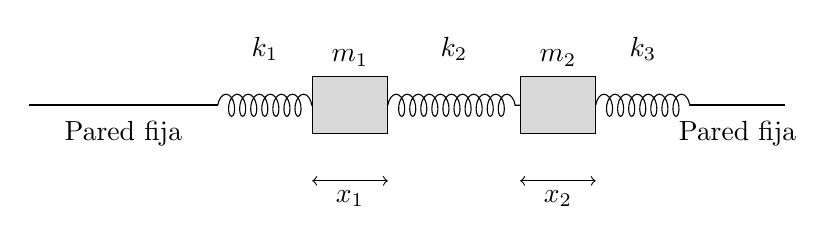
\begin{tikzpicture}[scale=1.2]
\draw[thick] (-3,0) -- (-1,0);
\draw[decorate,decoration={coil,amplitude=4pt,segment length=4pt}] (-1,0) -- (0,0);
\draw[fill=gray!30] (0,-0.3) rectangle (0.8,0.3);
\node at (0.4,0.5) {$m_1$};
\draw[decorate,decoration={coil,amplitude=4pt,segment length=4pt}] (0.8,0) -- (2.2,0);
\draw[fill=gray!30] (2.2,-0.3) rectangle (3,0.3);
\node at (2.6,0.5) {$m_2$};
\draw[decorate,decoration={coil,amplitude=4pt,segment length=4pt}] (3,0) -- (4,0);
\draw[thick] (4,0) -- (5,0);
\node at (-2,-0.3) {Pared fija};
\node at (4.5,-0.3) {Pared fija};
\node at (-0.5,0.6) {$k_1$};
\node at (1.5,0.6) {$k_2$};
\node at (3.5,0.6) {$k_3$};
\draw[<->] (0,-0.8) -- (0.8,-0.8) node[midway,below] {$x_1$};
\draw[<->] (2.2,-0.8) -- (3,-0.8) node[midway,below] {$x_2$};
\end{tikzpicture}
\end{center}

Las posiciones de equilibrio son $x_1=x_2=0$. Las ecuaciones de movimiento son
\[
\begin{aligned}
m_1 x_1'' &= -k_1 x_1 + k_2(x_2-x_1),\\
m_2 x_2'' &= -k_2(x_2-x_1) - k_3 x_2.
\end{aligned}
\]
Reescribimos como sistema de primer orden definiendo $v_1=x_1'$, $v_2=x_2'$:
\[
\begin{cases}
x_1'=v_1,\\
v_1'=\dfrac{-(k_1+k_2)}{m_1}x_1+\dfrac{k_2}{m_1}x_2,\\
x_2'=v_2,\\
v_2'=\dfrac{k_2}{m_2}x_1-\dfrac{k_2+k_3}{m_2}x_2.
\end{cases}
\]

\begin{example}[Sistema masa-resorte con dos masas]
Tomemos $m_1=m_2=1$, $k_1=k_3=2$, $k_2=1$. Resolver el sistema para las posiciones $x_1,x_2$.
\begin{myproof}
\textbf{Paso 1.} Ecuaciones:
\[
x_1''=-3x_1+x_2,\qquad x_2''=x_1-3x_2.
\]
En forma de sistema con $\mathbf{X}=(x_1,x_2,v_1,v_2)^T$:
\[
\mathbf{X}'=
\begin{pmatrix}
0&0&1&0\\
0&0&0&1\\
-3&1&0&0\\
1&-3&0&0
\end{pmatrix}\mathbf{X}.
\]

\textbf{Paso 2.} Podemos resolver el sistema de segundo orden. Sumando y restando:
\[
(x_1+x_2)''=-2(x_1+x_2),\qquad (x_1-x_2)''=-4(x_1-x_2).
\]
Luego
\[
x_1+x_2=A\cos(\sqrt{2}t)+B\sen(\sqrt{2}t),
\]
\[
x_1-x_2=C\cos(2t)+D\sen(2t).
\]

\textbf{Paso 3.} Despejar:
\[
x_1=\frac12[(x_1+x_2)+(x_1-x_2)],
\]
\[
x_2=\frac12[(x_1+x_2)-(x_1-x_2)].
\]

\textbf{Respuesta final:}
\[
\boxed{
x_1(t)=\frac12\left(A\cos(\sqrt{2}t)+B\sen(\sqrt{2}t)+C\cos(2t)+D\sen(2t)\right),
}
\]
\[
\boxed{
x_2(t)=\frac12\left(A\cos(\sqrt{2}t)+B\sen(\sqrt{2}t)-C\cos(2t)-D\sen(2t)\right).
}
\]
\end{myproof}
\end{example}

\subsection{Circuitos eléctricos con dos mallas}

Consideremos un circuito con dos mallas, cada una con una inductancia $L_i$, resistencia $R_i$ y una fuente de voltaje $E_i(t)$, acopladas por una inductancia mutua $M$ o una resistencia común. Para simplificar, tomamos el sistema de mallas con corrientes $i_1(t), i_2(t)$ que satisfacen
\[
\begin{aligned}
L_1 i_1' + R_1 i_1 + M i_2' &= E_1(t),\\
M i_1' + L_2 i_2' + R_2 i_2 &= E_2(t).
\end{aligned}
\]
Si $L_1L_2-M^2\neq 0$, podemos despejar las derivadas y obtener un sistema de primer orden.

\begin{example}[Circuito acoplado]
Sean $L_1=2$, $L_2=1$, $M=1$, $R_1=3$, $R_2=2$, $E_1(t)=0$, $E_2(t)=e^{-t}$. Plantear el sistema y resolver.
\begin{myproof}
\textbf{Paso 1.} Ecuaciones:
\[
2i_1'+i_2'+3i_1=0,\qquad i_1'+i_2'+2i_2=e^{-t}.
\]
Despejar $i_1', i_2'$. Restando la segunda de la primera: $(2i_1'+i_2'+3i_1)-(i_1'+i_2'+2i_2)= -e^{-t}$,
\[
i_1' + 3i_1 -2i_2 = -e^{-t}\Rightarrow i_1' = -3i_1+2i_2-e^{-t}.
\]
De la segunda: $i_2'=e^{-t}-i_1'-2i_2 = e^{-t}-(-3i_1+2i_2-e^{-t})-2i_2 = 3i_1 -4i_2+2e^{-t}$.

\textbf{Paso 2.} Sistema:
\[
\mathbf{I}'=
\begin{pmatrix}
-3&2\\
3&-4
\end{pmatrix}
\mathbf{I}
+
\begin{pmatrix}
-e^{-t}\\
2e^{-t}
\end{pmatrix}.
\]

\textbf{Paso 3.} Resolver homogéneo. Valores propios de $A$: $\det(A-\lambda I)=(-3-\lambda)(-4-\lambda)-6=\lambda^2+7\lambda+6=(\lambda+1)(\lambda+6)$. Raíces $\lambda=-1,-6$.
Vectores propios: para $\lambda=-1$: $(A+I)\mathbf{v}=0\Rightarrow
\begin{pmatrix}
-2&2\\
3&-3
\end{pmatrix}\Rightarrow v_1=v_2$, $\mathbf{v}_1=(1,1)^T$.
Para $\lambda=-6$: $(A+6I)\mathbf{v}=0\Rightarrow
\begin{pmatrix}
3&2\\
3&2
\end{pmatrix}\Rightarrow 3v_1+2v_2=0$, $\mathbf{v}_2=(2,-3)^T$.
Homogénea: $\mathbf{I}_h=c_1 e^{-t}(1,1)^T+c_2 e^{-6t}(2,-3)^T$.

\textbf{Paso 4.} Particular. Como $\mathbf{F}(t)=e^{-t}(-1,2)^T$ y $-1$ es valor propio, proponemos $\mathbf{I}_p=t e^{-t}\mathbf{a}+e^{-t}\mathbf{b}$.
Derivada: $\mathbf{I}_p'=e^{-t}[(t+1)\mathbf{a}+\mathbf{b}]$.
Sustituir:
\[
(t+1)\mathbf{a}+\mathbf{b}=A(t\mathbf{a}+\mathbf{b})+\begin{pmatrix}-1\\2\end{pmatrix}
\]
\[
\Rightarrow t(A\mathbf{a}-\mathbf{a})+(A\mathbf{b}-\mathbf{a}-\mathbf{b})+\begin{pmatrix}-1\\2\end{pmatrix}=0.
\]
Para $t$: $A\mathbf{a}=\mathbf{a}\Rightarrow \mathbf{a}$ vector propio para $\lambda=-1$: $\mathbf{a}=\alpha(1,1)^T$.
Independiente: $(A-I)\mathbf{b} = \mathbf{a} - \begin{pmatrix}-1\\2\end{pmatrix}
= \begin{pmatrix}\alpha+1\\ \alpha-2\end{pmatrix}$.
Resolvemos $(A-I)\mathbf{b}=
\begin{pmatrix}
-4&2\\
3&-5
\end{pmatrix}\mathbf{b}$.
Sistema:
\[
-4b_1+2b_2=\alpha+1,\quad 3b_1-5b_2=\alpha-2.
\]
Eliminamos: de la primera $b_2=(\alpha+1+4b_1)/2$. Sustituir en segunda:
$3b_1-5(\alpha+1+4b_1)/2=\alpha-2\Rightarrow 6b_1-5\alpha-5-20b_1=2\alpha-4\Rightarrow -14b_1=7\alpha+1\Rightarrow b_1=-(7\alpha+1)/14$.
Para consistencia elegimos $\alpha$ tal que no importe; cualquier $\alpha$ da solución. Tomamos $\alpha=1$, entonces $\mathbf{a}=(1,1)^T$,
$b_1=-(8)/14=-4/7$, $b_2=(\alpha+1+4b_1)/2=(2-16/7)/2=(14/7-16/7)/2=(-2/7)/2=-1/7$.
Luego $\mathbf{b}=(-4/7,-1/7)^T$.

\textbf{Paso 5.} Particular:
\[
\mathbf{I}_p=t e^{-t}\begin{pmatrix}1\\1\end{pmatrix}+e^{-t}\begin{pmatrix}-4/7\\-1/7\end{pmatrix}.
\]

\textbf{Respuesta final:}
\[
\boxed{
\mathbf{I}(t)=c_1 e^{-t}
\begin{pmatrix}
1\\1
\end{pmatrix}
+c_2 e^{-6t}
\begin{pmatrix}
2\\-3
\end{pmatrix}
+
e^{-t}
\begin{pmatrix}
t-\frac47\\
t-\frac17
\end{pmatrix}
}
\]
\end{myproof}
\end{example}

\subsection{Modelos de población: sistemas lineales de competencia}

El modelo linealizado de Lotka-Volterra o sistemas de competencia tienen la forma
\[
\begin{cases}
x' = a x + b y,\\
y' = c x + d y,
\end{cases}
\]
donde $x,y$ representan poblaciones (o desviaciones de un punto de equilibrio). La naturaleza del punto crítico $(0,0)$ se determina por los valores propios de la matriz.

\begin{example}[Modelo depredador-presa linealizado]
Dado el sistema
\[
\begin{cases}
x' = x - 2y,\\
y' = 3x - 4y,
\end{cases}
\]
clasificar el punto crítico y hallar la solución general.
\begin{myproof}
\textbf{Paso 1.} Matriz $A=
\begin{pmatrix}
1&-2\\
3&-4
\end{pmatrix}$. Valores propios:
\[
\det(A-\lambda I)=(1-\lambda)(-4-\lambda)+6 = \lambda^2+3\lambda+2=(\lambda+1)(\lambda+2).
\]
Raíces: $\lambda_1=-1,\; \lambda_2=-2$. Ambas negativas, por lo que el punto crítico es un \emph{nodo estable}.

\textbf{Paso 2.} Vectores propios:
Para $\lambda=-1$: $(A+I)\mathbf{v}=0\Rightarrow
\begin{pmatrix}
2&-2\\
3&-3
\end{pmatrix}\Rightarrow v_1=v_2$, $\mathbf{v}_1=(1,1)^T$.
Para $\lambda=-2$: $(A+2I)\mathbf{v}=0\Rightarrow
\begin{pmatrix}
3&-2\\
3&-2
\end{pmatrix}\Rightarrow 3v_1-2v_2=0$, $\mathbf{v}_2=(2,3)^T$.

\textbf{Paso 3.} Solución general:
\[
\mathbf{X}=c_1 e^{-t}\begin{pmatrix}1\\1\end{pmatrix}+c_2 e^{-2t}\begin{pmatrix}2\\3\end{pmatrix}.
\]

\textbf{Respuesta final:}
\[
\boxed{
\mathbf{X}(t)=c_1 e^{-t}
\begin{pmatrix}
1\\1
\end{pmatrix}
+c_2 e^{-2t}
\begin{pmatrix}
2\\3
\end{pmatrix},
\quad \text{el origen es un nodo estable.}
}
\]
\end{myproof}
\end{example}

\section{Problemas propuestos}

\begin{prob}
Convertir la EDO $y'''+2y''-5y'+y=\cos t$ en un sistema de primer orden.
\end{prob}
\begin{myproof}
Definir $x_1=y,\; x_2=y',\; x_3=y''$. Entonces:
\[
x_1'=x_2,\quad x_2'=x_3,\quad x_3'=-2x_3+5x_2-x_1+\cos t.
\]
Forma matricial:
\[
\boxed{
\mathbf{X}'=
\begin{pmatrix}
0&1&0\\
0&0&1\\
-1&5&-2
\end{pmatrix}
\mathbf{X}
+
\begin{pmatrix}
0\\0\\\cos t
\end{pmatrix}.
}
\]
\end{myproof}

\begin{prob}
Escribir el sistema asociado a $y^{(4)}-3y''+2y'= e^{2t}$.
\end{prob}
\begin{myproof}
Tomamos $x_1=y,\; x_2=y',\; x_3=y'',\; x_4=y'''$. Entonces:
\[
x_1'=x_2,\; x_2'=x_3,\; x_3'=x_4,\; x_4'=3x_3-2x_2+e^{2t}.
\]
Sistema:
\[
\boxed{
\mathbf{X}'=
\begin{pmatrix}
0&1&0&0\\
0&0&1&0\\
0&0&0&1\\
0&-2&3&0
\end{pmatrix}
\mathbf{X}
+
\begin{pmatrix}
0\\0\\0\\e^{2t}
\end{pmatrix}.
}
\]
\end{myproof}

\begin{prob}
Usar el método de eliminación para resolver:
\[
\begin{cases}
x'=2x+3y,\\
y'=x+2y.
\end{cases}
\]
\end{prob}
\begin{myproof}
De la primera, $y=(x'-2x)/3$. Derivando: $y'=(x''-2x')/3$. Sustituir en segunda:
\[
\frac{x''-2x'}{3}=x+2\frac{x'-2x}{3}=x+\frac{2x'-4x}{3}.
\]
Multiplicar por 3: $x''-2x'=3x+2x'-4x\Rightarrow x''-4x'+x=0$.
Ecuación característica: $r^2-4r+1=0\Rightarrow r=2\pm\sqrt{3}$.
Entonces $x(t)=c_1 e^{(2+\sqrt{3})t}+c_2 e^{(2-\sqrt{3})t}$.
\[
y=\frac{x'-2x}{3}=\frac{(2+\sqrt{3})c_1 e^{(2+\sqrt{3})t}+(2-\sqrt{3})c_2 e^{(2-\sqrt{3})t}-2x}{3}
=\frac{\sqrt{3}}{3}c_1 e^{(2+\sqrt{3})t}-\frac{\sqrt{3}}{3}c_2 e^{(2-\sqrt{3})t}.
\]
\[
\boxed{
x(t)=c_1 e^{(2+\sqrt{3})t}+c_2 e^{(2-\sqrt{3})t},\quad
y(t)=\frac{\sqrt{3}}{3}c_1 e^{(2+\sqrt{3})t}-\frac{\sqrt{3}}{3}c_2 e^{(2-\sqrt{3})t}.
}
\]
\end{myproof}

\begin{prob}
Resolver por eliminación:
\[
\begin{cases}
x'=x-y,\\
y'=x+3y.
\end{cases}
\]
\end{prob}
\begin{myproof}
$y=x-x'$, $y'=x'-x''$. Sustituir en $y'=x+3y$:
$x'-x''=x+3(x-x')=4x-3x'\Rightarrow x''-4x'+4x=0$.
Raíz doble: $r^2-4r+4=0\Rightarrow (r-2)^2=0\Rightarrow r=2$.
$x(t)=(c_1+c_2 t)e^{2t}$.
$y=x-x'=(c_1+c_2 t)e^{2t}-[c_2 e^{2t}+2(c_1+c_2 t)e^{2t}]=[-(c_1+c_2)-c_2 t]e^{2t}$.
\[
\boxed{
x(t)=(c_1+c_2 t)e^{2t},\quad
y(t)=-(c_1+c_2)e^{2t}-c_2 t e^{2t}.
}
\]
\end{myproof}

\begin{prob}
Resolver el sistema homogéneo $\mathbf{X}'=
\begin{pmatrix}
2&1\\
1&2
\end{pmatrix}\mathbf{X}$.
\end{prob}
\begin{myproof}
Valores propios: $\det(A-\lambda I)=(2-\lambda)^2-1=(\lambda-1)(\lambda-3)$. $\lambda_1=1,\lambda_2=3$.
Vectores propios: para $\lambda=1$: $(A-I)\mathbf{v}=0\Rightarrow v_1+v_2=0$, $\mathbf{v}_1=(1,-1)^T$. Para $\lambda=3$: $(A-3I)\mathbf{v}=0\Rightarrow -v_1+v_2=0$, $\mathbf{v}_2=(1,1)^T$.
Solución:
\[
\boxed{
\mathbf{X}(t)=c_1 e^t
\begin{pmatrix}
1\\-1
\end{pmatrix}
+c_2 e^{3t}
\begin{pmatrix}
1\\1
\end{pmatrix}.
}
\]
\end{myproof}

\begin{prob}
Resolver $\mathbf{X}'=
\begin{pmatrix}
2&0\\
1&3
\end{pmatrix}\mathbf{X}$.
\end{prob}
\begin{myproof}
Valores propios: $\lambda_1=2,\lambda_2=3$. Vectores: para $\lambda=2$: $(A-2I)\mathbf{v}=0\Rightarrow
\begin{pmatrix}
0&0\\1&1
\end{pmatrix}\Rightarrow v_1+v_2=0$, $\mathbf{v}_1=(1,-1)^T$. Para $\lambda=3$: $(A-3I)\mathbf{v}=0\Rightarrow
\begin{pmatrix}
-1&0\\1&0
\end{pmatrix}\Rightarrow v_1=0$, $\mathbf{v}_2=(0,1)^T$.
Solución:
\[
\boxed{
\mathbf{X}(t)=c_1 e^{2t}
\begin{pmatrix}
1\\-1
\end{pmatrix}
+c_2 e^{3t}
\begin{pmatrix}
0\\1
\end{pmatrix}.
}
\]
\end{myproof}

\begin{prob}
Resolver $\mathbf{X}'=
\begin{pmatrix}
1&-2\\
2&1
\end{pmatrix}\mathbf{X}$.
\end{prob}
\begin{myproof}
Valores propios: $\lambda=1\pm2i$. Vector propio para $\lambda=1+2i$: $(A-(1+2i)I)\mathbf{v}=0\Rightarrow
\begin{pmatrix}
-2i&-2\\
2&-2i
\end{pmatrix}\Rightarrow -2i v_1-2v_2=0\Rightarrow v_2=-i v_1$. Tomamos $\mathbf{v}=(1,-i)^T=(1,0)^T+i(0,-1)^T$. $\mathbf{u}=(1,0),\mathbf{w}=(0,-1)$.
Solución real:
\[
\boxed{
\mathbf{X}(t)=e^t\left(c_1
\begin{pmatrix}
\cos 2t\\ \sen 2t
\end{pmatrix}
+c_2
\begin{pmatrix}
-\sen 2t\\ \cos 2t
\end{pmatrix}\right).
}
\]
(Nota: la segunda componente de $\mathbf{u}$ es 0, y de $\mathbf{w}$ es -1, por lo que la combinación da las dos soluciones.)
\end{myproof}

\begin{prob}
Resolver $\mathbf{X}'=
\begin{pmatrix}
-1&2\\
-1&-1
\end{pmatrix}\mathbf{X}$.
\end{prob}
\begin{myproof}
Valores propios: $\lambda=-1\pm i\sqrt{2}$? Calculemos: $\det(A-\lambda I)=(-1-\lambda)^2+2=(\lambda+1)^2+2=0\Rightarrow \lambda=-1\pm i\sqrt{2}$.
Vector propio para $\lambda=-1+i\sqrt{2}$: $(A-(-1+i\sqrt{2})I)\mathbf{v}=0\Rightarrow
\begin{pmatrix}
-i\sqrt{2}&2\\
-1&-i\sqrt{2}
\end{pmatrix}\Rightarrow -i\sqrt{2}v_1+2v_2=0\Rightarrow v_2=\frac{i\sqrt{2}}{2}v_1$. Tomamos $v_1=2$, $v_2=i\sqrt{2}$. $\mathbf{v}=(2,0)^T+i(0,\sqrt{2})^T$. $\mathbf{u}=(2,0),\mathbf{w}=(0,\sqrt{2})$.
Solución:
\[
\boxed{
\mathbf{X}(t)=e^{-t}\left(c_1
\begin{pmatrix}
2\cos(\sqrt{2}t)\\
-\sqrt{2}\sen(\sqrt{2}t)
\end{pmatrix}
+c_2
\begin{pmatrix}
2\sen(\sqrt{2}t)\\
\sqrt{2}\cos(\sqrt{2}t)
\end{pmatrix}\right).
}
\]
\end{myproof}

\begin{prob}
Resolver $\mathbf{X}'=
\begin{pmatrix}
5&1\\
-1&3
\end{pmatrix}\mathbf{X}$.
\end{prob}
\begin{myproof}
Valores propios: $\det(A-\lambda I)=(5-\lambda)(3-\lambda)+1=\lambda^2-8\lambda+16=(\lambda-4)^2$.
Vector propio: $(A-4I)\mathbf{v}=0\Rightarrow
\begin{pmatrix}
1&1\\
-1&-1
\end{pmatrix}\Rightarrow v_1+v_2=0$, $\mathbf{v}=(1,-1)^T$.
Vector generalizado: $(A-4I)\mathbf{w}=\mathbf{v}\Rightarrow
\begin{pmatrix}
1&1\\
-1&-1
\end{pmatrix}\mathbf{w}=(1,-1)^T\Rightarrow w_1+w_2=1$. Elegimos $\mathbf{w}=(1,0)^T$.
Solución:
\[
\boxed{
\mathbf{X}(t)=e^{4t}\left(c_1
\begin{pmatrix}
1\\-1
\end{pmatrix}
+c_2\left(t
\begin{pmatrix}
1\\-1
\end{pmatrix}
+
\begin{pmatrix}
1\\0
\end{pmatrix}\right)\right)
=
e^{4t}
\begin{pmatrix}
c_1+c_2(t+1)\\
-c_1-c_2 t
\end{pmatrix}.
}
\]
\end{myproof}

\begin{prob}
Resolver $\mathbf{X}'=
\begin{pmatrix}
1&2&0\\
0&1&2\\
0&0&1
\end{pmatrix}\mathbf{X}$.
\end{prob}
\begin{myproof}
$\lambda=1$ triple. Vector propio $(A-I)\mathbf{v}=0\Rightarrow
\begin{pmatrix}
0&2&0\\
0&0&2\\
0&0&0
\end{pmatrix}\Rightarrow v_2=0,v_3=0$, $\mathbf{v}=(1,0,0)^T$.
$\mathbf{w}_1$: $(A-I)\mathbf{w}_1=\mathbf{v}\Rightarrow
\begin{cases}
2w_{1,2}=1\\
2w_{1,3}=0
\end{cases}
\Rightarrow w_{1,2}=1/2, w_{1,3}=0$, elegimos $w_{1,1}=0$, $\mathbf{w}_1=(0,1/2,0)^T$.
$\mathbf{w}_2$: $(A-I)\mathbf{w}_2=\mathbf{w}_1\Rightarrow
\begin{cases}
2w_{2,2}=0\\
2w_{2,3}=1/2
\end{cases}
\Rightarrow w_{2,2}=0, w_{2,3}=1/4$, elegimos $w_{2,1}=0$, $\mathbf{w}_2=(0,0,1/4)^T$.
Solución:
\[
\boxed{
\mathbf{X}(t)=e^t\left(c_1
\begin{pmatrix}
1\\0\\0
\end{pmatrix}
+c_2\left(t
\begin{pmatrix}
1\\0\\0
\end{pmatrix}
+
\begin{pmatrix}
0\\1/2\\0
\end{pmatrix}\right)
+c_3\left(\frac{t^2}{2}
\begin{pmatrix}
1\\0\\0
\end{pmatrix}
+t
\begin{pmatrix}
0\\1/2\\0
\end{pmatrix}
+
\begin{pmatrix}
0\\0\\1/4
\end{pmatrix}\right)\right).
}
\]
\end{myproof}

\begin{prob}
Resolver $\mathbf{X}'=
\begin{pmatrix}
1&2\\
-2&1
\end{pmatrix}\mathbf{X}
+
\begin{pmatrix}
0\\1
\end{pmatrix}$ por coeficientes indeterminados.
\end{prob}
\begin{myproof}
Homogénea: $\lambda=1\pm2i$, $\mathbf{X}_h=e^t(c_1(\cos2t,-\sen2t)^T+c_2(\sen2t,\cos2t)^T)$.
Particular constante $\mathbf{a}$: $A\mathbf{a}=-(0,1)^T\Rightarrow
\begin{pmatrix}
1&2\\
-2&1
\end{pmatrix}\mathbf{a}=(0,-1)^T$.
Resolviendo: $a_1+2a_2=0,\;-2a_1+a_2=-1$. De la primera $a_1=-2a_2$, sustituir: $4a_2+a_2=-1\Rightarrow a_2=-1/5,\; a_1=2/5$.
Solución:
\[
\boxed{
\mathbf{X}(t)=e^t\left(c_1
\begin{pmatrix}
\cos2t\\-\sen2t
\end{pmatrix}
+c_2
\begin{pmatrix}
\sen2t\\\cos2t
\end{pmatrix}\right)
+
\begin{pmatrix}
2/5\\-1/5
\end{pmatrix}.
}
\]
\end{myproof}

\begin{prob}
Resolver $\mathbf{X}'=
\begin{pmatrix}
2&0\\
0&3
\end{pmatrix}\mathbf{X}
+
\begin{pmatrix}
e^{2t}\\e^{3t}
\end{pmatrix}$ por coeficientes indeterminados.
\end{prob}
\begin{myproof}
Homogénea: $\mathbf{X}_h=c_1 e^{2t}(1,0)^T+c_2 e^{3t}(0,1)^T$.
Como $2$ y $3$ son valores propios, proponemos $\mathbf{X}_p=t e^{2t}\mathbf{a}+ t e^{3t}\mathbf{b}$.
Derivada: $\mathbf{X}_p'=e^{2t}(\mathbf{a}+2t\mathbf{a})+e^{3t}(\mathbf{b}+3t\mathbf{b})$.
Sustituir y separar:
Para $e^{2t}$: $\mathbf{a}+2t\mathbf{a}=A(t\mathbf{a})+\begin{pmatrix}1\\0\end{pmatrix}$? Mejor, como la matriz es diagonal, las ecuaciones son independientes:
$x'=2x+e^{2t}\Rightarrow x_p=t e^{2t}$.
$y'=3y+e^{3t}\Rightarrow y_p=t e^{3t}$.
Por tanto $\mathbf{X}_p=(t e^{2t}, t e^{3t})^T$.
Solución:
\[
\boxed{
\mathbf{X}(t)=c_1 e^{2t}
\begin{pmatrix}
1\\0
\end{pmatrix}
+c_2 e^{3t}
\begin{pmatrix}
0\\1
\end{pmatrix}
+
\begin{pmatrix}
t e^{2t}\\
t e^{3t}
\end{pmatrix}.
}
\]
\end{myproof}

\begin{prob}
Resolver $\mathbf{X}'=
\begin{pmatrix}
0&1\\
-1&0
\end{pmatrix}\mathbf{X}
+
\begin{pmatrix}
\tan t\\0
\end{pmatrix}$ mediante variación de parámetros.
\end{prob}
\begin{myproof}
$\Phi(t)=
\begin{pmatrix}
\cos t&\sen t\\
-\sen t&\cos t
\end{pmatrix}$, $\Phi^{-1}=
\begin{pmatrix}
\cos t&-\sen t\\
\sen t&\cos t
\end{pmatrix}$.
$\Phi^{-1}\mathbf{F}=
\begin{pmatrix}
\cos t&-\sen t\\
\sen t&\cos t
\end{pmatrix}
\begin{pmatrix}
\tan t\\0
\end{pmatrix}
=
\begin{pmatrix}
\sen t\\
\tan t\sen t
\end{pmatrix}
=
\begin{pmatrix}
\sen t\\
\frac{\sen^2 t}{\cos t}
\end{pmatrix}.
$
Integral: $\int \sen t\,dt = -\cos t$, $\int \frac{\sen^2 t}{\cos t}dt = \int \frac{1-\cos^2 t}{\cos t}dt = \int(\sec t-\cos t)dt = \ln|\sec t+\tan t|-\sen t$.
Particular:
\[
\mathbf{X}_p=\Phi
\begin{pmatrix}
-\cos t\\
\ln|\sec t+\tan t|-\sen t
\end{pmatrix}.
\]
Solución:
\[
\boxed{
\mathbf{X}(t)=c_1
\begin{pmatrix}
\cos t\\-\sen t
\end{pmatrix}
+c_2
\begin{pmatrix}
\sen t\\\cos t
\end{pmatrix}
+
\Phi
\begin{pmatrix}
-\cos t\\
\ln|\sec t+\tan t|-\sen t
\end{pmatrix}.
}
\]
\end{myproof}

\begin{prob}
( Aplicación masa-resorte ) Resolver el sistema de masas acopladas con $m_1=2,\; m_2=1,\; k_1=1,\; k_2=2,\; k_3=1$.
\end{prob}
\begin{myproof}
Ecuaciones:
\[
2x_1''= -x_1+2(x_2-x_1)= -3x_1+2x_2,\quad x_2''=-2(x_2-x_1)-x_2=2x_1-3x_2.
\]
Sistema: $\mathbf{X}''=
\begin{pmatrix}
-3/2&1\\
2&-3
\end{pmatrix}\mathbf{X}$.
Valores propios de la matriz de segundas derivadas: $\det(A-\lambda I)=(-3/2-\lambda)(-3-\lambda)-2 = \lambda^2+\frac92\lambda+\frac{9}{2}-2 = \lambda^2+\frac92\lambda+\frac52=0\Rightarrow 2\lambda^2+9\lambda+5=0\Rightarrow \lambda=\frac{-9\pm\sqrt{81-40}}{4}=\frac{-9\pm\sqrt{41}}{4}$.
Ambos negativos, así que las frecuencias son $\omega_1=\sqrt{-\lambda_1}$, $\omega_2=\sqrt{-\lambda_2}$. Solución vectorial:
\[
\boxed{
\mathbf{X}(t)=c_1
\begin{pmatrix}
1\\ v_{11}
\end{pmatrix}\cos(\omega_1 t)+c_2
\begin{pmatrix}
1\\ v_{11}
\end{pmatrix}\sen(\omega_1 t)
+c_3
\begin{pmatrix}
1\\ v_{21}
\end{pmatrix}\cos(\omega_2 t)+c_4
\begin{pmatrix}
1\\ v_{21}
\end{pmatrix}\sen(\omega_2 t)
}
\]
con los vectores propios correspondientes.
\end{myproof}

\begin{prob}
( Aplicación circuito ) Resolver el sistema de mallas con $L_1=1,\; L_2=1,\; M=0,\; R_1=2,\; R_2=3,\; E_1=0,\; E_2=5$.
\end{prob}
\begin{myproof}
Sin acoplamiento: $i_1'+2i_1=0\Rightarrow i_1=c_1 e^{-2t}$. $i_2'+3i_2=5\Rightarrow i_2=c_2 e^{-3t}+\frac53$.
Solución:
\[
\boxed{
i_1(t)=c_1 e^{-2t},\quad i_2(t)=c_2 e^{-3t}+\frac53.
}
\]
\end{myproof}

\begin{prob}
( Modelo de población ) Clasificar el punto crítico de
\[
\begin{cases}
x'=x+2y,\\
y'=2x+y.
\end{cases}
\]
\end{prob}
\begin{myproof}
$A=
\begin{pmatrix}
1&2\\
2&1
\end{pmatrix}$, valores propios $\lambda=3,-1$. Uno positivo, uno negativo, por tanto el origen es un \emph{punto silla}.
\end{myproof}

\begin{prob}
Resolver el sistema $\mathbf{X}'=
\begin{pmatrix}
1&2\\
2&1
\end{pmatrix}\mathbf{X}$ y clasificar.
\end{prob}
\begin{myproof}
$\lambda_1=3,\; \lambda_2=-1$. Vectores: para $\lambda=3$: $\mathbf{v}_1=(1,1)^T$; para $\lambda=-1$: $\mathbf{v}_2=(1,-1)^T$.
Solución:
\[
\boxed{
\mathbf{X}(t)=c_1 e^{3t}
\begin{pmatrix}
1\\1
\end{pmatrix}
+c_2 e^{-t}
\begin{pmatrix}
1\\-1
\end{pmatrix},\quad \text{punto silla.}
}
\]
\end{myproof}

\begin{prob}
Resolver $\mathbf{X}'=
\begin{pmatrix}
-1&4\\
-1&-1
\end{pmatrix}\mathbf{X}$
y clasificar.
\end{prob}
\begin{myproof}
Valores propios: $\det(A-\lambda I)=(-1-\lambda)^2+4=0\Rightarrow \lambda=-1\pm2i$. Parte real negativa, por lo que el origen es un \emph{foco estable}. Vector propio para $\lambda=-1+2i$: $(A-(-1+2i)I)\mathbf{v}=0\Rightarrow
\begin{pmatrix}
-2i&4\\
-1&-2i
\end{pmatrix}\Rightarrow -2i v_1+4v_2=0\Rightarrow v_2=\frac{i}{2}v_1$. Tomamos $v_1=2$, $v_2=i$, $\mathbf{v}=(2,0)^T+i(0,1)^T$.
Solución:
\[
\boxed{
\mathbf{X}(t)=e^{-t}\left(c_1
\begin{pmatrix}
2\cos 2t\\
-\sen 2t
\end{pmatrix}
+c_2
\begin{pmatrix}
2\sen 2t\\
\cos 2t
\end{pmatrix}\right).
}
\]
\end{myproof}

\begin{prob}
Resolver $\mathbf{X}'=
\begin{pmatrix}
1&1\\
-1&1
\end{pmatrix}\mathbf{X}$
y clasificar.
\end{prob}
\begin{myproof}
$\lambda=1\pm i$. Parte real positiva, origen es un \emph{foco inestable}. Vector propio para $\lambda=1+i$: $(A-(1+i)I)\mathbf{v}=0\Rightarrow
\begin{pmatrix}
-i&1\\
-1&-i
\end{pmatrix}\Rightarrow -i v_1+v_2=0\Rightarrow v_2=i v_1$. Tomamos $v_1=1$, $v_2=i$, $\mathbf{v}=(1,0)^T+i(0,1)^T$.
Solución:
\[
\boxed{
\mathbf{X}(t)=e^t\left(c_1
\begin{pmatrix}
\cos t\\-\sen t
\end{pmatrix}
+c_2
\begin{pmatrix}
\sen t\\\cos t
\end{pmatrix}\right).
}
\]
\end{myproof}

\begin{prob}
Resolver $\mathbf{X}'=
\begin{pmatrix}
0&-1\\
1&0
\end{pmatrix}\mathbf{X}$
y clasificar.
\end{prob}
\begin{myproof}
$\lambda=\pm i$, parte real cero, origen es un \emph{centro}. Solución:
\[
\boxed{
\mathbf{X}(t)=c_1
\begin{pmatrix}
\cos t\\\sen t
\end{pmatrix}
+c_2
\begin{pmatrix}
-\sen t\\\cos t
\end{pmatrix}.
}
\]
\end{myproof}

